
%(BEGIN_QUESTION)
% Copyright 2010, Tony R. Kuphaldt, released under the Creative Commons Attribution License (v 1.0)
% This means you may do almost anything with this work of mine, so long as you give me proper credit

Examine this ``live'' display of a Siemens S7-300 PLC's program, and from this determine all bit statuses represented by the color highlighting in this ladder logic program:

$$\includegraphics[width=15.5cm]{i01873x01.eps}$$

\begin{itemize}
\item{} {\tt I0.2} = ???
\vskip 10pt
\item{} {\tt I0.5} = ???
\vskip 10pt
\item{} {\tt I1.1} = ???
\vskip 10pt
\item{} {\tt Q0.1} = ???
\vskip 10pt
\item{} {\tt Q0.6} = ???
\end{itemize}

\underbar{file i01873}
%(END_QUESTION)





%(BEGIN_ANSWER)

\begin{itemize}
\item{} {\tt I0.2} = 0
\item{} {\tt I0.5} = 1
\item{} {\tt I1.1} = 0
\item{} {\tt Q0.1} = 1
\item{} {\tt Q0.6} = 0
\end{itemize}

%(END_ANSWER)





%(BEGIN_NOTES)


%INDEX% PLC, relating I/O status to virtual elements 

%(END_NOTES)


